\section{Classic Mechanics}
\subsection{Formulations}
we call the description of a given theory in a particular mathematical arena a formulation of the theory.

\textbf{Lagrangian}
$$
L=T-V
$$
where $T$ denotes the kinetic energy and $V$ the potential energy.

\textbf{Euler-Lagrange equation}
$$
\frac{\partial L}{\partial q}-\frac{d}{d t}\left(\frac{\partial L}{\partial \dot{q}}\right)=0
$$

\textbf{Hamiltonian}
$$
H=p \dot{q}-L
$$
where $p$ denotes the momentum, $\dot{q}$ the velocity and $L,$ as before,
the Lagrangian. 

\textbf{Hamiltonian's equation}
$$
\begin{array}{l}{\frac{d p}{d t}=-\frac{\partial H}{\partial q}} \\ {\frac{d q}{d t}=\frac{\partial H}{\partial p}}\end{array}
$$

\textbf{Summary}

\tikzset{every picture/.style={line width=0.75pt}} %set default line width to 0.75pt        

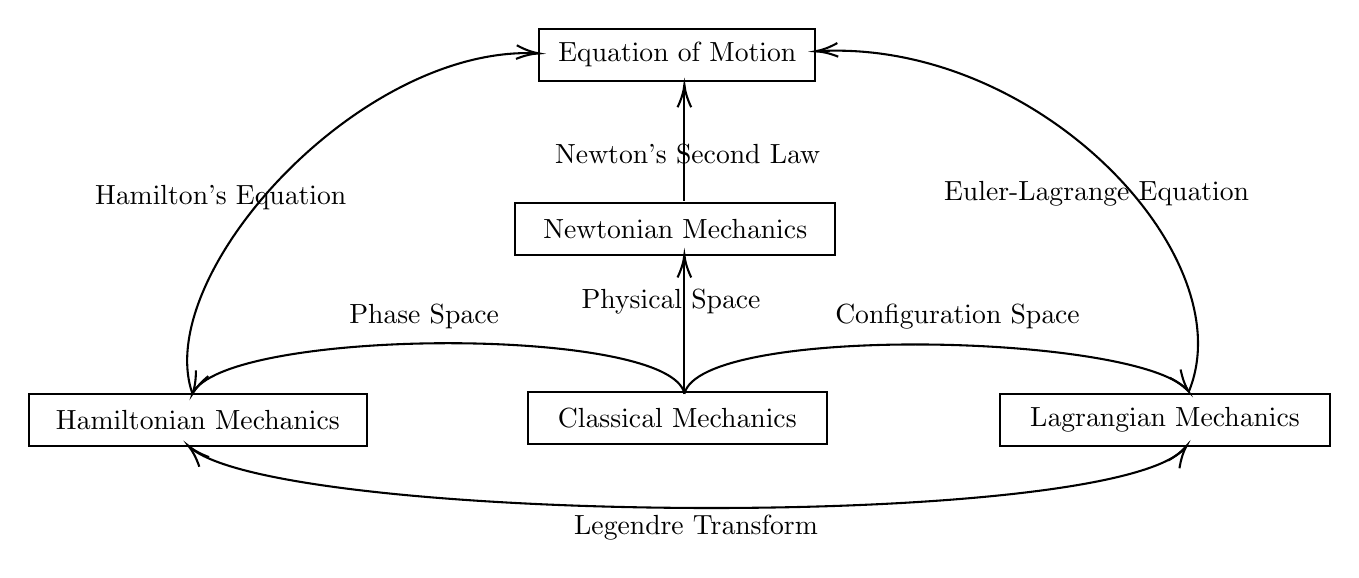
\begin{tikzpicture}[x=0.75pt,y=0.75pt,yscale=-1,xscale=1]
%uncomment if require: \path (0,300); %set diagram left start at 0, and has height of 300

%Straight Lines [id:da6596978253438757] 
\draw    (319.4,108.4) -- (319.4,54.4) ;
\draw [shift={(319.4,52.4)}, rotate = 450] [color={rgb, 255:red, 0; green, 0; blue, 0 }  ][line width=0.75]    (10.93,-3.29) .. controls (6.95,-1.4) and (3.31,-0.3) .. (0,0) .. controls (3.31,0.3) and (6.95,1.4) .. (10.93,3.29)   ;

%Straight Lines [id:da9635704269170282] 
\draw    (319.4,201.4) -- (319.4,136.4) ;
\draw [shift={(319.4,134.4)}, rotate = 450] [color={rgb, 255:red, 0; green, 0; blue, 0 }  ][line width=0.75]    (10.93,-3.29) .. controls (6.95,-1.4) and (3.31,-0.3) .. (0,0) .. controls (3.31,0.3) and (6.95,1.4) .. (10.93,3.29)   ;

%Curve Lines [id:da8601213705090224] 
\draw    (319.4,201.4) .. controls (313.49,168.89) and (103.83,169.38) .. (83.21,199.98) ;
\draw [shift={(82.4,201.4)}, rotate = 295.11] [color={rgb, 255:red, 0; green, 0; blue, 0 }  ][line width=0.75]    (10.93,-3.29) .. controls (6.95,-1.4) and (3.31,-0.3) .. (0,0) .. controls (3.31,0.3) and (6.95,1.4) .. (10.93,3.29)   ;

%Curve Lines [id:da5496082538732877] 
\draw    (319.4,201.4) .. controls (327.28,167.91) and (535.03,172.26) .. (561.33,199.16) ;
\draw [shift={(562.4,200.4)}, rotate = 233.13] [color={rgb, 255:red, 0; green, 0; blue, 0 }  ][line width=0.75]    (10.93,-3.29) .. controls (6.95,-1.4) and (3.31,-0.3) .. (0,0) .. controls (3.31,0.3) and (6.95,1.4) .. (10.93,3.29)   ;

%Curve Lines [id:da6432080478617446] 
\draw    (82.33,228.09) .. controls (129.49,264.15) and (525.01,267.7) .. (560.44,227.63) ;
\draw [shift={(561.4,226.4)}, rotate = 484.44] [color={rgb, 255:red, 0; green, 0; blue, 0 }  ][line width=0.75]    (10.93,-3.29) .. controls (6.95,-1.4) and (3.31,-0.3) .. (0,0) .. controls (3.31,0.3) and (6.95,1.4) .. (10.93,3.29)   ;
\draw [shift={(80.4,226.4)}, rotate = 45.61] [color={rgb, 255:red, 0; green, 0; blue, 0 }  ][line width=0.75]    (10.93,-3.29) .. controls (6.95,-1.4) and (3.31,-0.3) .. (0,0) .. controls (3.31,0.3) and (6.95,1.4) .. (10.93,3.29)   ;
%Curve Lines [id:da7865585332239224] 
\draw    (82.4,201.4) .. controls (62.5,144.68) and (162.39,33.52) .. (248.11,37.33) ;
\draw [shift={(249.4,37.4)}, rotate = 183.33] [color={rgb, 255:red, 0; green, 0; blue, 0 }  ][line width=0.75]    (10.93,-3.29) .. controls (6.95,-1.4) and (3.31,-0.3) .. (0,0) .. controls (3.31,0.3) and (6.95,1.4) .. (10.93,3.29)   ;

%Curve Lines [id:da532295931617982] 
\draw    (562.4,200.4) .. controls (589.26,135.72) and (490.4,30.46) .. (384,36.3) ;
\draw [shift={(382.4,36.4)}, rotate = 356.26] [color={rgb, 255:red, 0; green, 0; blue, 0 }  ][line width=0.75]    (10.93,-3.29) .. controls (6.95,-1.4) and (3.31,-0.3) .. (0,0) .. controls (3.31,0.3) and (6.95,1.4) .. (10.93,3.29)   ;



% Text Node
\draw (325,266) node   [align=left] {Legendre Transform};
% Text Node
\draw (194,164) node   [align=left] {Phase Space};
% Text Node
\draw (451,164) node   [align=left] {Configuration Space};
% Text Node
\draw (313,157) node   [align=left] {Physical Space};
% Text Node
\draw (96,107) node   [align=left] {Hamilton's Equation};
% Text Node
\draw (518,105) node   [align=left] {Euler-Lagrange Equation};
% Text Node
\draw (321,86) node   [align=left] {Newton's Second Law};
% Text Node
\draw    (3.5,201.5) -- (166.5,201.5) -- (166.5,226.5) -- (3.5,226.5) -- cycle  ;
\draw (85,214) node   [align=left] {Hamiltonian Mechanics};
% Text Node
\draw    (244,200.5) -- (388,200.5) -- (388,225.5) -- (244,225.5) -- cycle  ;
\draw (316,213) node   [align=left] {Classical Mechanics};
% Text Node
\draw    (471.5,201.5) -- (630.5,201.5) -- (630.5,226.5) -- (471.5,226.5) -- cycle  ;
\draw (551,214) node   [align=left] {Lagrangian Mechanics};
% Text Node
\draw    (238,109.5) -- (392,109.5) -- (392,134.5) -- (238,134.5) -- cycle  ;
\draw (315,122) node   [align=left] {Newtonian Mechanics};
% Text Node
\draw    (249.5,25.5) -- (382.5,25.5) -- (382.5,50.5) -- (249.5,50.5) -- cycle  ;
\draw (316,38) node   [align=left] {Equation of Motion};


\end{tikzpicture}

\subsection{Basic quantities}
\textbf{Momentum} is the velocity of an object times its mass
$$
\vec{p}(t) \equiv m \dot{\vec{q}}(t)
$$
$$
\begin{array}{c}{\frac{d p}{d t}=F} \\ {\int_{t_{i}}^{t_{f}} d p=\int_{t_{i}}^{t_{f}} F d t} \\ {\Delta p=F \Delta t}\end{array}
$$
\textbf{In words, this means that the momentum of an object tells
us how long it takes a given force $F$ to stop it. Formulated
differently, we need a much bigger force to stop it quickly.}

\textbf{Angular momentum} is defined as the cross product of the position vector and the momentum vector
$$
\vec{L}(t)=\vec{q}(t) \times \vec{p}(t)=m \vec{q}(t) \times \dot{q}(t)
$$
While (linear) momentum tells us how hard it
is to stop an object using a specific force, angular momentum tells us how hard it is to stop it spinning.

\textbf{Momentum and angular momentum are conserved.}